\documentclass[border=8pt]{standalone}
\usepackage{tikz}
\usepackage{xcolor}
\usetikzlibrary{positioning}

\definecolor{mlpinput}{RGB}{131,109,169}   % primary purple   (input layer)
\definecolor{mlphidA}{RGB}{167,149,196}    % light purple     (hidden 1)
\definecolor{mlphidB}{RGB}{61,146,140}     % teal accent      (hidden 2)
\definecolor{mlpout}{RGB}{51,159,52}       % green            (output)
\definecolor{mlpedge}{RGB}{170,170,170}    % light grey edges
\definecolor{mlpstroke}{RGB}{90,90,90}

\begin{document}
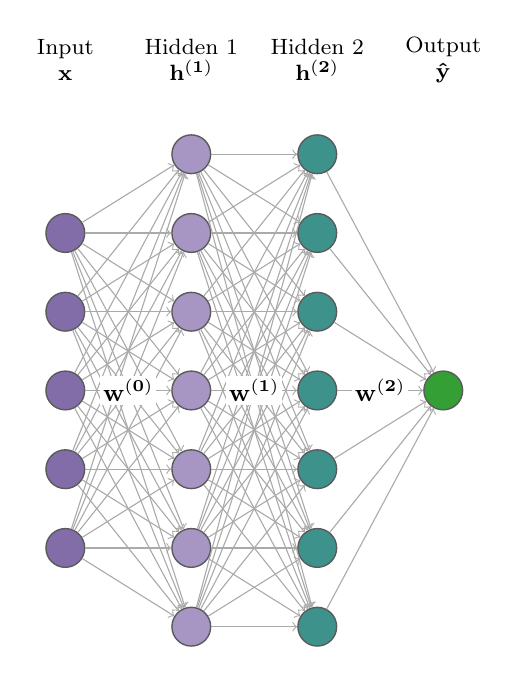
\begin{tikzpicture}[
    x=1.6cm, y=1.0cm,
    node distance=1cm,
    neuron/.style={draw=mlpstroke, circle, minimum size=14pt, inner sep=0pt, line width=0.5pt},
    every node/.style={font=\small},
]
  \node[neuron, fill=mlpinput] (n0_0) at (0,2.0) {};
  \node[neuron, fill=mlpinput] (n0_1) at (0,1.0) {};
  \node[neuron, fill=mlpinput] (n0_2) at (0,0.0) {};
  \node[neuron, fill=mlpinput] (n0_3) at (0,-1.0) {};
  \node[neuron, fill=mlpinput] (n0_4) at (0,-2.0) {};
  \node[neuron, fill=mlphidA] (n1_0) at (1,3.0) {};
  \node[neuron, fill=mlphidA] (n1_1) at (1,2.0) {};
  \node[neuron, fill=mlphidA] (n1_2) at (1,1.0) {};
  \node[neuron, fill=mlphidA] (n1_3) at (1,0.0) {};
  \node[neuron, fill=mlphidA] (n1_4) at (1,-1.0) {};
  \node[neuron, fill=mlphidA] (n1_5) at (1,-2.0) {};
  \node[neuron, fill=mlphidA] (n1_6) at (1,-3.0) {};
  \node[neuron, fill=mlphidB] (n2_0) at (2,3.0) {};
  \node[neuron, fill=mlphidB] (n2_1) at (2,2.0) {};
  \node[neuron, fill=mlphidB] (n2_2) at (2,1.0) {};
  \node[neuron, fill=mlphidB] (n2_3) at (2,0.0) {};
  \node[neuron, fill=mlphidB] (n2_4) at (2,-1.0) {};
  \node[neuron, fill=mlphidB] (n2_5) at (2,-2.0) {};
  \node[neuron, fill=mlphidB] (n2_6) at (2,-3.0) {};
  \node[neuron, fill=mlpout] (n3_0) at (3,0.0) {};
  \draw[->, mlpedge, line width=0.4pt] (n0_0) -- (n1_0);
  \draw[->, mlpedge, line width=0.4pt] (n0_0) -- (n1_1);
  \draw[->, mlpedge, line width=0.4pt] (n0_0) -- (n1_2);
  \draw[->, mlpedge, line width=0.4pt] (n0_0) -- (n1_3);
  \draw[->, mlpedge, line width=0.4pt] (n0_0) -- (n1_4);
  \draw[->, mlpedge, line width=0.4pt] (n0_0) -- (n1_5);
  \draw[->, mlpedge, line width=0.4pt] (n0_0) -- (n1_6);
  \draw[->, mlpedge, line width=0.4pt] (n0_1) -- (n1_0);
  \draw[->, mlpedge, line width=0.4pt] (n0_1) -- (n1_1);
  \draw[->, mlpedge, line width=0.4pt] (n0_1) -- (n1_2);
  \draw[->, mlpedge, line width=0.4pt] (n0_1) -- (n1_3);
  \draw[->, mlpedge, line width=0.4pt] (n0_1) -- (n1_4);
  \draw[->, mlpedge, line width=0.4pt] (n0_1) -- (n1_5);
  \draw[->, mlpedge, line width=0.4pt] (n0_1) -- (n1_6);
  \draw[->, mlpedge, line width=0.4pt] (n0_2) -- (n1_0);
  \draw[->, mlpedge, line width=0.4pt] (n0_2) -- (n1_1);
  \draw[->, mlpedge, line width=0.4pt] (n0_2) -- (n1_2);
  \draw[->, mlpedge, line width=0.4pt] (n0_2) -- (n1_3);
  \draw[->, mlpedge, line width=0.4pt] (n0_2) -- (n1_4);
  \draw[->, mlpedge, line width=0.4pt] (n0_2) -- (n1_5);
  \draw[->, mlpedge, line width=0.4pt] (n0_2) -- (n1_6);
  \draw[->, mlpedge, line width=0.4pt] (n0_3) -- (n1_0);
  \draw[->, mlpedge, line width=0.4pt] (n0_3) -- (n1_1);
  \draw[->, mlpedge, line width=0.4pt] (n0_3) -- (n1_2);
  \draw[->, mlpedge, line width=0.4pt] (n0_3) -- (n1_3);
  \draw[->, mlpedge, line width=0.4pt] (n0_3) -- (n1_4);
  \draw[->, mlpedge, line width=0.4pt] (n0_3) -- (n1_5);
  \draw[->, mlpedge, line width=0.4pt] (n0_3) -- (n1_6);
  \draw[->, mlpedge, line width=0.4pt] (n0_4) -- (n1_0);
  \draw[->, mlpedge, line width=0.4pt] (n0_4) -- (n1_1);
  \draw[->, mlpedge, line width=0.4pt] (n0_4) -- (n1_2);
  \draw[->, mlpedge, line width=0.4pt] (n0_4) -- (n1_3);
  \draw[->, mlpedge, line width=0.4pt] (n0_4) -- (n1_4);
  \draw[->, mlpedge, line width=0.4pt] (n0_4) -- (n1_5);
  \draw[->, mlpedge, line width=0.4pt] (n0_4) -- (n1_6);
  \draw[->, mlpedge, line width=0.4pt] (n1_0) -- (n2_0);
  \draw[->, mlpedge, line width=0.4pt] (n1_0) -- (n2_1);
  \draw[->, mlpedge, line width=0.4pt] (n1_0) -- (n2_2);
  \draw[->, mlpedge, line width=0.4pt] (n1_0) -- (n2_3);
  \draw[->, mlpedge, line width=0.4pt] (n1_0) -- (n2_4);
  \draw[->, mlpedge, line width=0.4pt] (n1_0) -- (n2_5);
  \draw[->, mlpedge, line width=0.4pt] (n1_0) -- (n2_6);
  \draw[->, mlpedge, line width=0.4pt] (n1_1) -- (n2_0);
  \draw[->, mlpedge, line width=0.4pt] (n1_1) -- (n2_1);
  \draw[->, mlpedge, line width=0.4pt] (n1_1) -- (n2_2);
  \draw[->, mlpedge, line width=0.4pt] (n1_1) -- (n2_3);
  \draw[->, mlpedge, line width=0.4pt] (n1_1) -- (n2_4);
  \draw[->, mlpedge, line width=0.4pt] (n1_1) -- (n2_5);
  \draw[->, mlpedge, line width=0.4pt] (n1_1) -- (n2_6);
  \draw[->, mlpedge, line width=0.4pt] (n1_2) -- (n2_0);
  \draw[->, mlpedge, line width=0.4pt] (n1_2) -- (n2_1);
  \draw[->, mlpedge, line width=0.4pt] (n1_2) -- (n2_2);
  \draw[->, mlpedge, line width=0.4pt] (n1_2) -- (n2_3);
  \draw[->, mlpedge, line width=0.4pt] (n1_2) -- (n2_4);
  \draw[->, mlpedge, line width=0.4pt] (n1_2) -- (n2_5);
  \draw[->, mlpedge, line width=0.4pt] (n1_2) -- (n2_6);
  \draw[->, mlpedge, line width=0.4pt] (n1_3) -- (n2_0);
  \draw[->, mlpedge, line width=0.4pt] (n1_3) -- (n2_1);
  \draw[->, mlpedge, line width=0.4pt] (n1_3) -- (n2_2);
  \draw[->, mlpedge, line width=0.4pt] (n1_3) -- (n2_3);
  \draw[->, mlpedge, line width=0.4pt] (n1_3) -- (n2_4);
  \draw[->, mlpedge, line width=0.4pt] (n1_3) -- (n2_5);
  \draw[->, mlpedge, line width=0.4pt] (n1_3) -- (n2_6);
  \draw[->, mlpedge, line width=0.4pt] (n1_4) -- (n2_0);
  \draw[->, mlpedge, line width=0.4pt] (n1_4) -- (n2_1);
  \draw[->, mlpedge, line width=0.4pt] (n1_4) -- (n2_2);
  \draw[->, mlpedge, line width=0.4pt] (n1_4) -- (n2_3);
  \draw[->, mlpedge, line width=0.4pt] (n1_4) -- (n2_4);
  \draw[->, mlpedge, line width=0.4pt] (n1_4) -- (n2_5);
  \draw[->, mlpedge, line width=0.4pt] (n1_4) -- (n2_6);
  \draw[->, mlpedge, line width=0.4pt] (n1_5) -- (n2_0);
  \draw[->, mlpedge, line width=0.4pt] (n1_5) -- (n2_1);
  \draw[->, mlpedge, line width=0.4pt] (n1_5) -- (n2_2);
  \draw[->, mlpedge, line width=0.4pt] (n1_5) -- (n2_3);
  \draw[->, mlpedge, line width=0.4pt] (n1_5) -- (n2_4);
  \draw[->, mlpedge, line width=0.4pt] (n1_5) -- (n2_5);
  \draw[->, mlpedge, line width=0.4pt] (n1_5) -- (n2_6);
  \draw[->, mlpedge, line width=0.4pt] (n1_6) -- (n2_0);
  \draw[->, mlpedge, line width=0.4pt] (n1_6) -- (n2_1);
  \draw[->, mlpedge, line width=0.4pt] (n1_6) -- (n2_2);
  \draw[->, mlpedge, line width=0.4pt] (n1_6) -- (n2_3);
  \draw[->, mlpedge, line width=0.4pt] (n1_6) -- (n2_4);
  \draw[->, mlpedge, line width=0.4pt] (n1_6) -- (n2_5);
  \draw[->, mlpedge, line width=0.4pt] (n1_6) -- (n2_6);
  \draw[->, mlpedge, line width=0.4pt] (n2_0) -- (n3_0);
  \draw[->, mlpedge, line width=0.4pt] (n2_1) -- (n3_0);
  \draw[->, mlpedge, line width=0.4pt] (n2_2) -- (n3_0);
  \draw[->, mlpedge, line width=0.4pt] (n2_3) -- (n3_0);
  \draw[->, mlpedge, line width=0.4pt] (n2_4) -- (n3_0);
  \draw[->, mlpedge, line width=0.4pt] (n2_5) -- (n3_0);
  \draw[->, mlpedge, line width=0.4pt] (n2_6) -- (n3_0);
  \node[align=center, font=\footnotesize] at (0,4.20) {Input\\$\mathbf{x}$};
  \node[align=center, font=\footnotesize] at (1,4.20) {Hidden 1\\$\mathbf{h^{(1)}}$};
  \node[align=center, font=\footnotesize] at (2,4.20) {Hidden 2\\$\mathbf{h^{(2)}}$};
  \node[align=center, font=\footnotesize] at (3,4.20) {Output\\$\mathbf{\hat{y}}$};
  \node[fill=white, inner sep=1pt] at (0.5,0) {$\mathbf{w^{(0)}}$};
  \node[fill=white, inner sep=1pt] at (1.5,0) {$\mathbf{w^{(1)}}$};
  \node[fill=white, inner sep=1pt] at (2.5,0) {$\mathbf{w^{(2)}}$};
\end{tikzpicture}
\end{document}
